%% LyX 1.6.2 created this file.  For more info, see http://www.lyx.org/.
%% Do not edit unless you really know what you are doing.
\documentclass[12pt,english]{article}
\usepackage{mathptmx}
\renewcommand{\familydefault}{\rmdefault}
\usepackage[T1]{fontenc}
\usepackage[latin9]{inputenc}
\usepackage[letterpaper]{geometry}
\geometry{verbose,tmargin=2cm,bmargin=2cm,lmargin=2cm,rmargin=2cm,headheight=1cm,headsep=1cm,footskip=1cm}
\setlength{\parskip}{\medskipamount}
\setlength{\parindent}{0pt}
\usepackage{graphicx}

\usepackage{babel}

\begin{document}

\part*{Chemie}


\section*{Der Blei-Akkumulator}


\subsection*{Entladevorgang}

Negativer Pol (Anode, Oxidation):

\[
Pb+SO_{4}^{2-}\rightarrow PbSO_{4}+2e^{-}\]


Positiver Pol (Kathode, Reduktion):

\[
PbO_{2}+SO_{4}^{2-}+4H_{3}O^{+}+2e^{-}\rightarrow PbSO_{4}+6H_{2}O\]


Gesamtreaktion:

\[
Pb+PbO_{2}+2H_{2}SO_{4}\rightarrow2PbSO_{4}+2H_{2}O\]


\bigskip{}


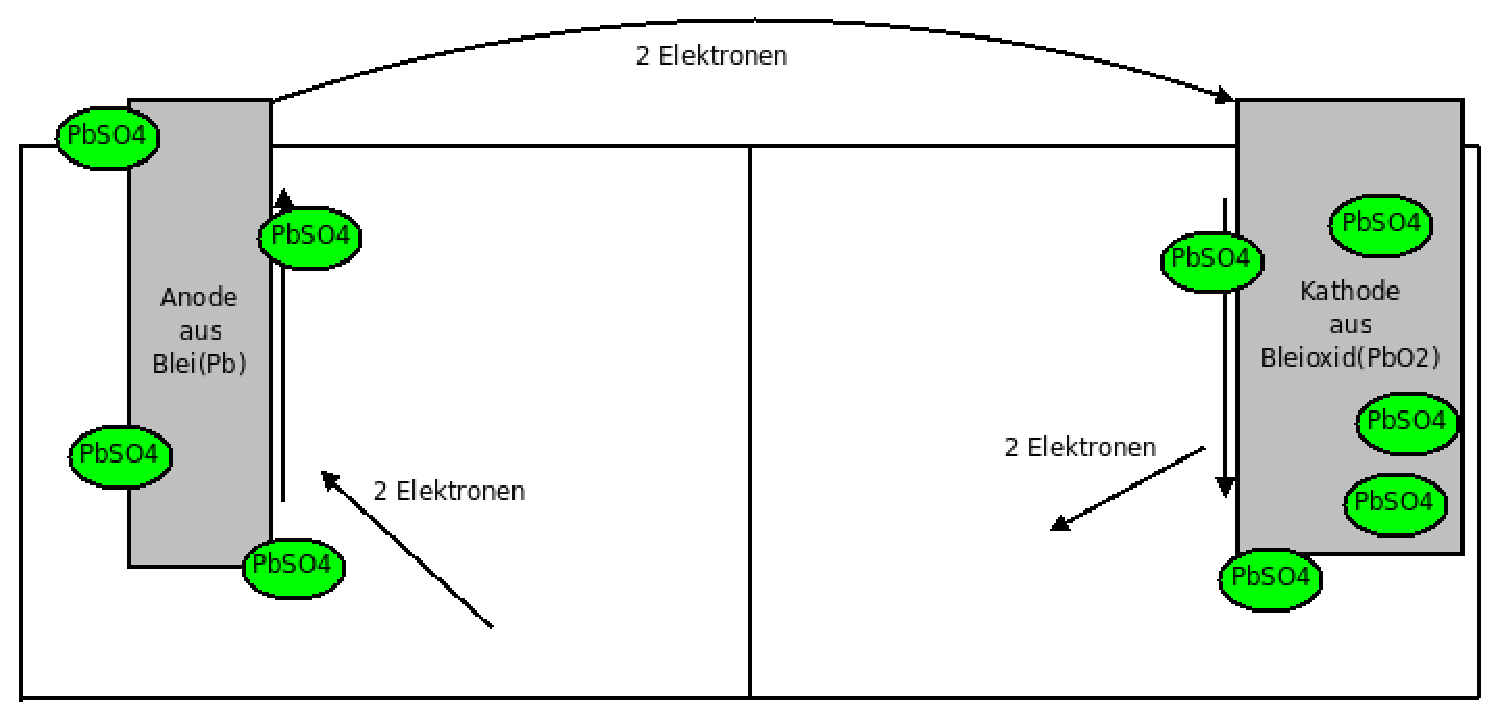
\includegraphics[scale=0.7]{Endladen}

\newpage{}


\subsection*{Ladevorgang}

Negativer Pol (Anode, Oxidation):

\[
PbSO_{4}+2e^{-}\rightarrow Pb+SO_{4}^{2-}\]


Positiver Pol (Kathode, Reduktion):

\[
PbSO_{4}+6H_{2}O\rightarrow PbO_{2}+SO_{4}^{2-}+4H_{3}O^{+}+2e^{-}\]


Gesamtreaktion:

\[
2PbSO_{4}+2H_{2}O\rightarrow Pb+PbO_{2}+2H_{2}SO_{4}\]


\bigskip{}


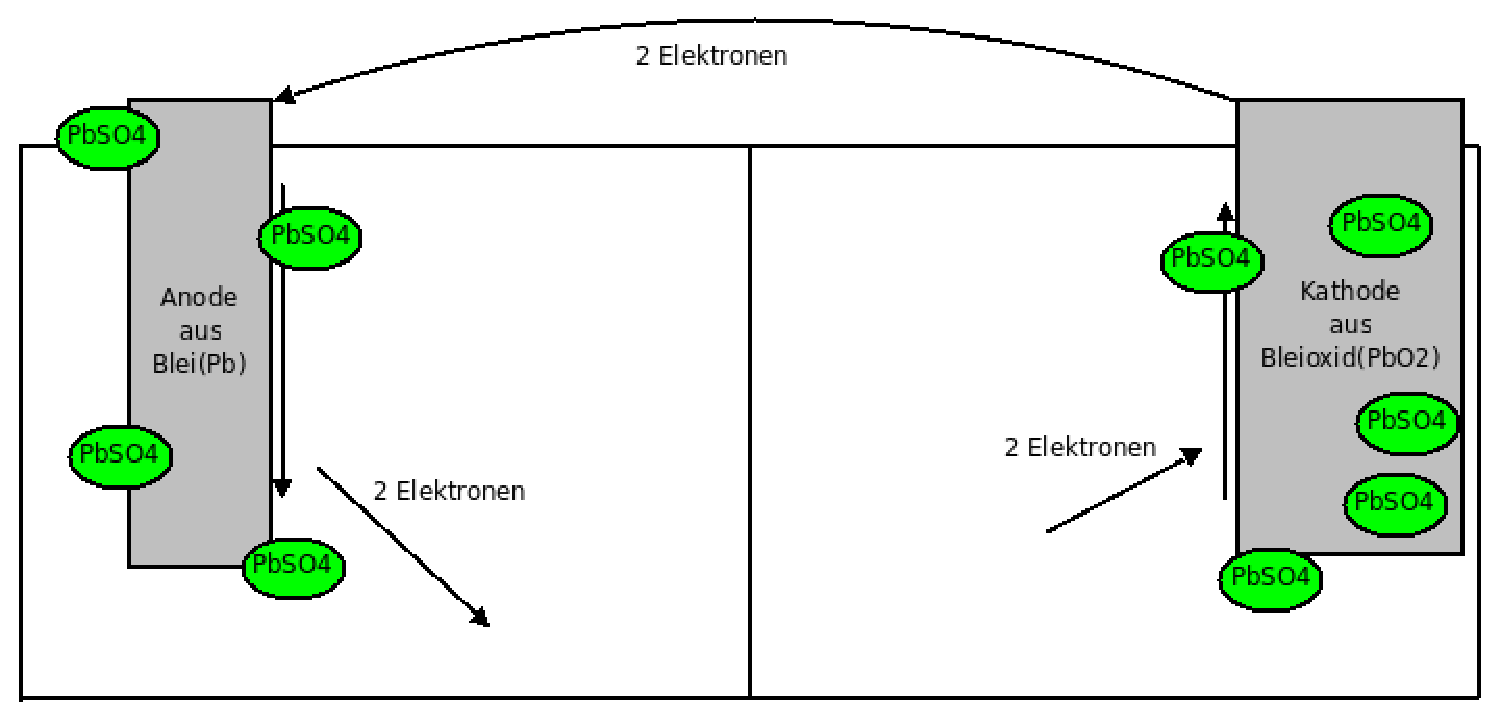
\includegraphics[scale=0.7]{Laden}
\end{document}
